\documentclass[10pt,a4paper]{article}
\usepackage[utf8]{inputenc}
\usepackage[english]{babel}
\usepackage{amsmath}
\usepackage{amsfonts}
\usepackage{amssymb}
\usepackage{makeidx}
\usepackage{graphicx}
\usepackage{array}
\usepackage{eurosym}
\usepackage{tabularx}
\usepackage{fancyhdr} %remove this to get rid of header/footer except pagenum
\author{Biggest}
\title{Shoppatomic (WORKING TITLE)}
\graphicspath{ {images/} }
\pagestyle{fancy} %remove this to get rid of header/footer except pagenum
\lhead{Shoppatomic} %replace or remove me (with game name?)
\lfoot{Biggest (c)}%replace or remove me (with company name?)
\begin{document}
% cover page
\maketitle
\newpage
% toc
\tableofcontents
\newpage
% main body

\begin{abstract}
%describe the goals of this document in a few paragraphs. Do you want it to simply outline the game for development purposes? Do you want to use it to pitch the idea to someone else? Do you need it as a guideline for writers and other staff? Furthermore, analyse the game in a short matter. List the purpose of the game, what will be fun about it, how the player character generally works (First/Third person? Movement? etc.) what the user can expect from it/what you expect to get from it etc. Keep it short! There is plenty of room to describe details later on
This document aims to outline the game to be created for all development purposes in enough detail to properly guide and aid in development. The document may be updated as development proceeds, however it is intended to lead development and therefore should be only updated with good reason. "Gunpowder Dream", henceforth referred to as "the game", is a story-driven single player first-person-shooter game with a focus on a host of alternative movement mechanics and strange weaponry. It follows a convenience store employee who has to complete a myriad of "special tasks", assigned to him by his employer randomly during his shift. 
\end{abstract}
\newpage




\section{Overview}
\subsection{Mission Statement}
%Describe the game in 1-2 sentences, similar to a shorthand descriptions you see on some online game retailers. It should be made intriging and informative. 
Welcome to "---come up with new name ----". Your job is to stack shelves, keep the store clean and handle any special tasks your boss needs. And don't worry, we have plenty of tools to handle whatever he throws at you. With your help we will become the most successful convenience store around! 
\subsection{Features}
%List some features here. Think of it as if you had to put all of these on the back of your games box. For each major feature, make a subsection and expand it a little with a few more bulletpoints
\begin{itemize}
 \item TODO TODO TODO TODO TODO TODO TODO TODO TODO TODO TODO TODO 
\end{itemize}
\subsection{Genres / Tags}
%Many storefronts have a variety of genres and tags to choose from. List any tags or genres you may apply to this game. Keep to well known and general tags like "First person shooter", "Singleplayer", "Shoot-em-up", "Sandbox", "VR-Support" etc. This helps give the reader a general understanding of what the game will be similar to, as well as lists some outstanding broad features, like multiplayer/co-op/vr support. 
\begin{itemize}
\item Single-Player
\item First-Person-Shooter
\item Story
\item Indie
\end{itemize}

\subsection{The "Ws"}
%Common questions someone may ask you/themselves when they hear about your game. Answer in a way that makes it sound intriguing, but make sure to always be as informative as possible. This is not meant to be only marketing, but rather provide a overview of some common aspects of your game in a way that is natural  and generally easier and more exciting to read than a long-form game analysis
\subsubsection{What is it?}
%Single paragraph explanation of the game
The game is about traversing a convenience store employee's dreams as he completes special tasks given to him by his employer throughout the storyline.
\subsubsection{Where does it take place?}
%Describe the setting (General World, Timesetting if applicable etc. Just paint a picture of what the world looks like with details that are important to the visual look or gameplay of your game in 1-2 paragraphs.
It takes place on Earth, in a rarely-visited stylised convenience store of the late 90s. The "dream-world", which the player gets transported to in certain cases, usually is a abstract version of a convenience store without much logic (infinite isles and nonsensical color patterns for example.)
\subsubsection{What am I controlling in the game?}
%Describe the player in broad strokes. Does it follow an excisting type of player (FPS-Player, 2D-Sidescrolling etc.)? How does it control? What is the camera-perspective used? etc. You may include some character details if you want but there is a section later to include as many traits as you want.
You control a unnamed first-person protagonist. You are able to walk around, interact with certain objects, pick up props, go through your inventory of "tools" and use these tools on the environment and enemies . The controls can be described as "FPS-Standard".
\subsubsection{What is the main goal?}
%If applicable, describe the final goal of the player. May be something like "reaching the end of the storyline" or some other arbitrary goal. May be multiple goals if the game has multiple gamemodes or has sidecontent that can be optionally completed etc.
Reaching the end of the storyline.
\subsubsection{What does the game focus on?}
%Main focus of your game. Commonly something like Story, Gameplay, Multiplayer Casual, Multiplayer Competitive or a mix. Can also be loosely defined, however make sure it remains informal and doesn't beat around the bush. 
The game mainly focuses on creative and unusual weapons, usually involving movement in a 3D space. It can be described as a linear PvE shooter sandbox with a storyline.
\subsubsection{Why did you make it?}
%Simple answer(s) only. May be something like "I like 3D shooters" or "I really wanted to try something new with a First Person game" or "I had a great idea for a story" but also something more complex and detailed like "I found the idea of moving through a level using only swinging ropes to be very interesting, so I wanted to pursue it further". This is free-form, only see what I am saying as a suggestion. Just keep it informative
I found that I genuinely enjoy fast-paced movement that many old-school arena shooters have and wanted to make a game that focused on weird gun and movement mechanics while also having some sort of "sensible" linear story.
\subsubsection{How is your game different to similar titles?}
%chances are your game follows some tropes or maybe even is a copy of an existing game. How is it different?
TODO TODO TODO
(Singleplayer =/= multiplayer?, more focus on movement?)
\subsection{Principles}
%use this section to list off generalised design goals for your game. These can be measureable or non-measureable and serve to further detail the understanding of the game concept, as well as fixate core principles you want your team/yourself to stick to while working. You may order them by priority if you want, or leave them unordered. These are very free form, however I recommend using them to fixate core design principles you want to stick to during development. Strinking a balance with measureability is also recommended. Furthermore, make sure that these principles are able to be followed during a long development cycle. Specifying that every level should have at least one easteregg is fine, while specifying that there must be exactly 324 estereggs in the game may be too specific and hard to follow. For example
\subsubsection{Goal \#1: Creativity with 3D-movement}
This game will try to be as creative with movement as possible. It will center around movement in a 3D environment for most of its game mechanic and level design.
\subsubsection{Goal \#2: Distinct roles for each weapon}
No weapon should technically be able to occupy the same role as another. There should not be a weapon that is fundamentally the same as another just with different weapons. Furthermore, the role contributed to the players inventory must be meaningful. Including a fully-automatic rifle just because there isnt one yet doesn't work if a fully-automatic rifle does not add anything meaningful to the gameplay. 
\subsubsection{Goal \#3: Lorem ipsum}
Lorem ipsum dolor sit amet, consectetur adipiscing elit, sed do eiusmod tempor incididunt ut labore et dolore magna aliqua. Ut enim ad minim veniam, quis nostrud exercitation ullamco laboris nisi ut aliquip ex ea commodo consequat.
\subsubsection{Target Audience}
%Who is this game for? Are you targeting a specific age group? What common traits do you think most of them will share? Likes/Dislikes, habits etc. Are you targeting fans of a specific genre or specific kind of other media? Are you targeting people from specific communities? 
This game will target fans of business and cooking simulators, as well as people who are interested in exploration and scavenging-type games. Furthermore, it will appeal to fans of indie-games and non-mainstream gameplay styles. Finally, the cartoon-inspired artstyle will target creative personality types and younger individuals alike. \\
Lorem ipsum dolor sit amet, consectetur adipiscing elit, sed do eiusmod tempor incididunt ut labore et dolore magna aliqua. Ut enim ad minim veniam, quis nostrud exercitation ullamco laboris nisi ut aliquip ex ea commodo consequat.

This game will target fans of movement shooters, single player games and indie games in general. It will be available as donationware (with free download as an option) to minimise the bar for entry. Furthermore, it targets other game developers by being open source, which allows for modified games and spinoffs using a simple fork of the repository. 

%-----------------------------------------
\section{Storyline}
\subsection{Synopsis}
%Write a short synopsis of your storyline. If your storyline is very complex, this may be longer, but it should be possible to use 500 Words or less, if not much less (around 100-200 for simple stories). Tips: Make character names bold when you first introduce them to make navigating easier. Include a character thumbnail as well when you first introduce them or shortly after (e.g. \textbf{Steven Smith}, (35), an Accountant for Bigbrown INC. - bland, unaffectionate, introverted and slender as a stick - ...). Keep language informative and neutral. Write in third person. Do not try to sell your story in your synopsis. It should serve as a summary of the story, not as a advertisement of it. If you want advertisement, come up with a 2-3 sentence starter-paragraph and put it at the very top before actually starting the synopsis. If you are having trouble shortening your (already written) story or if you are still writing it, you could try taking your basic structure (e.g. chaptertitles or sectiontitltes) and add storybeats to them in the order they appear in, until you have a detailed enough synopsis to convey the most important characteristics of the entire storyline. You can also try putting emphasis on important objects as tehy appear.

\emph{Player}, unnamed employee of \emph{"yume's convinience store"} - daydreamer, always tired and always wears a white suit-shirt with rolled up sleeves - tries to get through his daily chores but is always \emph{interrupted by his \emph{boss}}, unnamed unknown identity unknown age. He doesn't know his \emph{bosses} name as the original owner died long ago, but every-time the \emph{boss} calls, there is more work to do. The story begins on a regular work week, a monday. There isn't much to do, just stacking some shelves and picking up some trash from the floor. The \emph{boss} calls and instructs the \emph{player} to go out back and receive a special delivery that will arrive shortly, explaining that the \emph{boss} is expecting demand for a few products to spike soon and that he is taking a gamble. As the player opens the door to the storage-room, which he has to pass through to get to the delivery area, he finds himself stuck in another one of his day dreams. He has been having these uncontrollable day-dreams more frequently recently, probably caused by his lack of sleep getting worse. And its usually pretty similar to this one. The \emph{players} hands are turned to machine and he finds himself fighting robots as he tries to reach the end of the impossibly long storage room. The \emph{player} doesn't mind these dreams, since he finds them quite fun. Suddenly he is jumped by one of the enemies hiding in the lockers but as he goes to push the enemy away he finds himself pushing open the back room door to the delivery area.


TODO TODO TODO TODO
Lorem ipsum dolor sit amet, consectetur adipiscing elit, sed do eiusmod tempor incididunt ut labore et dolore magna aliqua. Quam vulputate dignissim suspendisse in est ante in nibh mauris. Est lorem ipsum dolor sit amet consectetur. Blandit massa enim nec dui nunc mattis. Eget nunc scelerisque viverra mauris in aliquam sem fringilla. Morbi blandit cursus risus at ultrices mi tempus imperdiet. Bibendum at varius vel pharetra vel turpis nunc. Integer feugiat scelerisque varius morbi enim nunc faucibus a. Ut pharetra sit amet aliquam id diam maecenas ultricies mi. Varius morbi enim nunc faucibus a pellentesque sit. Imperdiet dui accumsan sit amet nulla facilisi morbi tempus iaculis. Morbi non arcu risus quis varius quam. Viverra nibh cras pulvinar mattis nunc sed blandit libero volutpat. Non enim praesent elementum facilisis leo. Est velit egestas dui id ornare arcu odio ut. Potenti nullam ac tortor vitae purus faucibus ornare suspendisse sed. Proin sagittis nisl rhoncus mattis rhoncus urna neque viverra. Morbi quis commodo odio aenean sed adipiscing.

Amet consectetur adipiscing elit ut. Urna nec tincidunt praesent semper feugiat. Eleifend donec pretium vulputate sapien nec. Elementum nibh tellus molestie nunc non blandit massa enim. Mauris ultrices eros in cursus turpis massa tincidunt. Eget nulla facilisi etiam dignissim diam quis enim. Iaculis urna id volutpat lacus. Nulla porttitor massa id neque. Potenti nullam ac tortor vitae purus faucibus ornare suspendisse sed. Massa sed elementum tempus egestas sed. Orci phasellus egestas tellus rutrum tellus pellentesque eu tincidunt. Senectus et netus et malesuada fames ac turpis egestas.

Quis risus sed vulputate odio ut enim blandit volutpat maecenas. In massa tempor nec feugiat nisl pretium fusce id. Rhoncus urna neque viverra justo nec. Pretium nibh ipsum consequat nisl vel pretium lectus. Egestas erat imperdiet sed euismod. Elementum tempus egestas sed sed risus pretium. Cursus in hac habitasse platea dictumst quisque. Augue interdum velit euismod in pellentesque massa placerat duis. Sagittis purus sit amet volutpat consequat mauris nunc congue nisi. Risus nec feugiat in fermentum. Eros in cursus turpis massa tincidunt dui.


\subsection{Characters}
\subsubsection{Lorem Mc Ipsum}
\label{BOSS1}
\begin{center}

\includegraphics[width=2cm]{chartest} \\
\textbf{Name}:\\
Lorem Mc Ipsum\\
\textbf{Relations:}\\
\textbf{Player}: Interactable NPC. Tells short story and offers to sell various stabbing knives. \\
\textbf{Steve Fakename}: Brother of Fakename Ipsum. They have been competitive with eachother since birth. Lorem always wanted to best his brother in the stabbing competitions \\
\textbf{Traits:}\\
helpful\\
competitive\\
dealmaker\\
\textbf{MISC}:\\
MISC
\end{center}

%-----------------------------------------
\section{Gameplay}
\subsection{Core}
%Short 1-2 paragraph detail of the core gameplay. imagine you are trying to sum it up for a press release or a storefront description, just without the marketing. 
The player traverses the world using various tools to access normally unreachable places (such as high ledges). He collects various cooking and baking ingredients, as well as a wide variety of processed foods. Items collected can be used to produce product or directly used as product for the storefront. The storefront is a customisable restaurant, where the player has to manage customer interest, manage employees. as well as produce and serve food
\subsubsection{Modes}
%Quickly list the available gamemodes with a very short description. Replace with tabular or sections if modes need more explanation. However, if the general idea is as simple as seen below, the details will be filled in below.
\begin{itemize}
	\item \textbf{Story} - Singleplayer storymode
	\item \textbf{Multiplayer CO-OP Story} - Multiplayer storymode
	\item \textbf{Arena} - Arena PvP mode
	\item \textbf{Sandbox} - Sandbox exploration mode with "cheat-menu"
\end{itemize}
\subsection{Mechanics}
%detail all major game mechanics. headline of subsubsection is one line description / title of mechanic. Include a description of each mechanic that paints a complete picture, including what it does, how the player utilises/interacts with it, benefits the player gets from this mechanics (if applicable), drawbacks the player gets from this mechanic (if applicable), mistakes the player can make when dealing with the mechanic. Note that these are just suggestions. My tip is to think of it like you are writing a manual and you need to make sure that the user has a good understanding of what they are dealing with, what they have to do and what they shouldnt do. If you struggle to come up with a good long list of mechanics then either your game is a walking simulator or you should try and rethink some core game concepts. This section is definately one you should spend a lot of time on. Also try to find a standardised set of informations you want to provide for each mechanic. Some basic things you should write here are character movement ( if applicable ), items/tools/inventory (if applicable), camera logic (how the camera works. if your game has a complex camera make sure to describe it in a lot of detail), physical properties of the player (if applicable), other properties of the player (if applicable), level loading and level changes and some logistical features if they have a major impact on gameplay (like a matchmaking system in a multiplayer game). This would also be a good place to detail any UI that is a direct part of gameplay. General user interface stuff like main menus etc. can be detailed in the UX section.
\subsubsection{Character Movement}
\label{Character Movement}
The \emph{player} may move forward, backward, left, right (henceforth referred to as \emph{ground plane movement}), up and down (henceforth referred to as \emph{lateral movement}.

\emph{Ground Plane Movement} is achieved using conventional first person movement controls (WASD for Keyboards, Control Stick for controllers). The player usually walks at a fixed  top speed of 4 Units/s. However, the player may hold a designated \emph{run button} to move at a top speed of 6 Units/s. Movement speed above 6 Units/s is considered "sliding" and will drastically limit the control the player has over movement direction and speed until the velocity passes under this threshold by the means of friction or colliding with a wall. Speeds above this limit should not be able to be achieved by the player on his own, but rather must come from tool use or external forces acting on the player. \emph{sliding movement} is roughly 1/5th as effective as regular \emph{ground plane movement}

\emph{Lateral movement} can only be controlled by the player in the "up"-direction. Hitting a designated \emph{jump button} will cause the player to jump up using a fixed amount of force. Movement in the "down" direction is facilitated by the means of gravity. When not on the ground the player is in a \emph{falling} state, severely limiting his ability to change direction and accelerate, effectively limiting his \emph{Ground plane movement}. This \emph{air movement} is equivalent to 1/10th in strength compared to the regular \emph{Ground plane movement}.

\subsubsection{Character World Interactions}
\label{Character World Interactions}
The \emph{player} may be moved by \emph{physics props} when colliding with them. Collisions add to the internal momentum value of the player, respecting a simulated amount of mass. The force is then returned to the impacting object in a realistic way, preventing it from moving the player freely and allowing the player to also push around physics props. The player itself is not a fully simulated physics prop, but rather a script-controlled physics entity. Therefore, these interactions must be made possible in code. 

\subsubsection{Camera}
%I got a bit tired here. This should be way more precise. You have to be detailed enough that some developer who never played a video game before could implement this mechanic the way youd want it implemented. Even if something is convention, you should still explain it. Leaving things too open for interpretation here can lead to confusion and refactoring. Also I didnt bother looking up the actual names for these axis. You should really do that in your own document to avoid confusion and angry plane enthusiasts
The \emph{Camera} is a conventional mouse-look-based first-person-camera. As such, moving the mouse up, causes the camera to rotate up. Moving the mouse left, causes the camera to rotate left etc. 

\emph{Mouse sensitivity} can be configured in the games settings menu. Furthermore, the mouse directions may be \emph{inverted}, causing the camera to rotate in the opposite direction of what it would normally.

The cameras angles are clamped at 90DEG up/down on the up/down axis to prevent the player looking behind himself without turning around.

Rotating the camera left/right causes the players body to rotate with the camera.

Equipped tools are parented to the camera, making their viewmodels always appear in front of the camera.


%These were just two examples. They could be, and mabye should be, even more detailed. Also there should be a lot more mechanics. However, this is just an example using a made up video game.
\subsection{POV}
%Describe the players point of view. Include the literal Point of View (first person, third person etc.), what they control, how they traverse levels/interact with objects etc. Basically try to paint a picture of how the player will experience your game
Lorem ipsum dolor sit amet, consectetur adipiscing elit, sed do eiusmod tempor incididunt ut labore et dolore magna aliqua. Eu volutpat odio facilisis mauris. Quam pellentesque nec nam aliquam sem. Vel eros donec ac odio tempor orci dapibus. Morbi tristique senectus et netus. At auctor urna nunc id cursus metus aliquam. Volutpat sed cras ornare arcu dui. Interdum velit laoreet id donec ultrices tincidunt arcu non. Donec ultrices tincidunt arcu non sodales neque sodales ut etiam. Aliquam faucibus purus in massa. Etiam erat velit scelerisque in dictum non consectetur. Facilisis volutpat est velit egestas dui id. At erat pellentesque adipiscing commodo elit at imperdiet. Sit amet consectetur adipiscing elit duis. Libero id faucibus nisl tincidunt eget nullam non nisi. Tristique et egestas quis ipsum suspendisse. Non enim praesent elementum facilisis leo vel fringilla est ullamcorper. Est ullamcorper eget nulla facilisi etiam. Mattis rhoncus urna neque viverra justo nec ultrices. Facilisi nullam vehicula ipsum a arcu cursus vitae congue.

Quis varius quam quisque id diam vel quam. Dui ut ornare lectus sit amet. Habitant morbi tristique senectus et netus et malesuada. Ultricies tristique nulla aliquet enim tortor at auctor urna. Augue neque gravida in fermentum et sollicitudin ac orci. Consectetur lorem donec massa sapien faucibus et molestie ac feugiat. Duis convallis convallis tellus id interdum. Fames ac turpis egestas sed tempus urna. Ac odio tempor orci dapibus ultrices in iaculis nunc. Eget nulla facilisi etiam dignissim diam quis. Odio euismod lacinia at quis risus sed vulputate odio. Auctor augue mauris augue neque gravida in. Sit amet risus nullam eget felis eget nunc lobortis. Proin gravida hendrerit lectus a. Odio ut sem nulla pharetra diam sit amet nisl suscipit. 
\subsection{Objectives}
%Every game needs some objectives. List as many as you need. Consider splitting it into different sections. A good idea is to make a section for every game-style that your game includes (e.g. "Open World", "Baloon Minigame", "Trading Minigame", "Special Bossfight 1") or multiple generalised sections (e.g. "Per Level" / "Overarching"). 
\subsubsection{Per Level}
%Objective -> whats the objective
%Required For -> why does the player need to complete this objective
%Reward -> what does the player gain from the objective being completed
%Factors -> what factors does the players progress for this objective depend on
\begin{tabularx}{12cm}{|>{\raggedright\arraybackslash}X|>{\raggedright\arraybackslash}X|>{\raggedright\arraybackslash}X|>{\raggedright\arraybackslash}X|}
\hline
\textbf{Objective} & \textbf{Required For} & \textbf{Reward} & \textbf{Factors}\\
\hline
Collect Min. Amount Items & Finishing Open-World Section & Collected Items & Ability in Traversing Level; Puzzle-solving ability; Avoiding Environmental hazards \\
\hline
Make rent & Passing store management section & Passing to next level/day & Customer patience; Customer Interest; Employee Performance; Cost of bought equipment\\
\hline
\end{tabularx}
\subsubsection{Overarching}
\begin{tabularx}{12cm}{|>{\raggedright\arraybackslash}X|>{\raggedright\arraybackslash}X|>{\raggedright\arraybackslash}X|>{\raggedright\arraybackslash}X|}
\hline
\textbf{Objective} & \textbf{Required For} & \textbf{Reward} & \textbf{Factors}\\
\hline
Complete upgrade tree & 100\% game & Upgraded business performance; higher completion percentage & Resources required to upgrade; resources gained in a given period of time; order and efficiency of upgrades chosen \\
\hline
Reach last day & beat base game & Unlock infinite after-game section; complete base game & You have to pass all previous days / make rent consistently\\
\hline
\end{tabularx}

\subsection{Restrictions, Principles and Rules}
%List off a set of guidelines, rules and principles that the gameplay needs to adhere to at all times. These are important for development and must be followed. Rules and principles should also be intuitive so that a player can learn them on their own while playing. Failture to create intuitive rules/principles for your gameplay or failture to adhere to them, may make your game frustrating and unpredictable to play. It also increases the risk of your game design regressing in development or multiple teammembers disagreeing on various aspects of the gameplay. These rules should apply to all gamemodes. If they don't, consider indicating what mode they are for. The number of principles should be enough to pin down a consistent gameplay experience but not too many that development becomes slow or impossible. Unfortunately, this is something you need to judge for yourself.
\subsubsection{Standardised \& Expected Controls for First-Person elements}
Controls for the first-person controlled elements (walking, running, jumping, camera rotation, tool use) should follow the industry standard control schemes seen in products featuring a similar basic player archetype. This should be true for keyboard/mouse controls, as well as various controller control schemes, unless reconfigured by the player
\subsubsection{Prop intractability}
Objects in the game world should not be static, unless absolutely necessary to facility a playable gameplay performance or prevent unfixable physics bugs. Objects should be able to be picked up, moved and thrown if they are expected to be lift-able by a human being. Throws and picking up should reflect the simulated weight of the object that is being carried. Objects that cannot be carried should still react to physical interactions (e.g. a non-lift-able cast iron table being hit with a heavy lift-able object should still move as expected from a real simulated object of the respective weight).
\subsection{Mapping}
%List off the available maps/levels your game has. If you want, you can organise these as a node tree to visualise transitions or just use the template below and make a new section for each entry. 
\subsubsection{Tomato Town}
%Template for a single level info-table. If possible, make a sketch that includes the rough layout of your level with some marked spots that are very important. Note that this doesn't need to be accurate, but you may find it useful to visualise the idea you have for your level in a practical way before actually implementing it. You can also insert a screenshot of your level after you prototyped it or built a first version of it, or draw a logo or something. Or just leave it out. Write a short description of your map. Suggestions for stuff to put in the description: Style/Looks/Location/Time, Goal, Difficulty and "gimmick" if it has any. Can sound a bit like an advertisement or something youd put in a flyer. 
\begin{center}
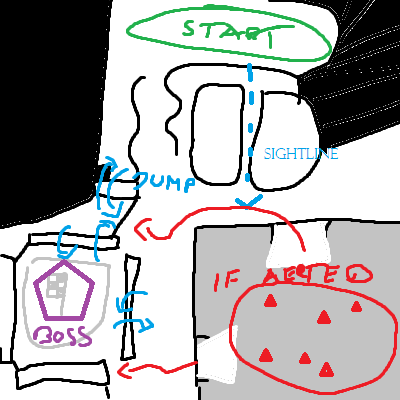
\includegraphics[scale=0.5]{map}\\

\textbf{Name:}\\
Tomato Town\\

\textbf{Description:}\\
Ten kills on the board rn, just wiped out tomato town.
Closed off arena. Defeat the boss and capture the item to win. A enemy base at night, located in sandy planes with many sightlines and cover to hide behind. Don't trigger the alarm, or you will be flooded with enemies. \\

\textbf{Hazards:}\\
%List the most important hazards the player will have to avoid on this map. If there is a special hazard, like a boss, consider linking to its character entry
\begin{itemize}
\item Don't trigger the alarm
\item Enemies are in the base
\item Boss fight at goal (non-avoidable) (\ref{BOSS1})
\end{itemize}
\textbf{Mechanics used:}\\
%list all mechanics used in this map. only use mechanics already detailed in this document. It would be a good idea to also add references to the references mechanics (omitted for most of them here since this is fake and I was too dumb to make a level that fits with the game ive been inventing so far)
\begin{itemize}
\item Character Movement (\ref{Character Movement})
\item Character Interactions (\ref{Character World Interactions})
\item Barrier Leap
\item Stealth
\item Alterable guards
\item Base-wide alerting
\end{itemize}

\textbf{Speciality:}\\
%describe what makes this map special. if there is a gimmick or a new mechanic thats first introduced, this is the place to show it/them off.
First stealth map in the game
\end{center}
%-----------------------------------------
\section{Aesthetics}
%this section details design principles and literal asthetic concepts/design details
\subsection{Principles}
%similar to game design principles. write down a set of rules, guidelines or principles your game should follow asthetically. if you find it hard to explain, consider including reference images. This may include pure artistic guidelines (limited color palette, limited sprite resolution, character proportions, menu styles, etc.) or gameplay-affecting asthetic choices (interactable objects flash when the player gets close etc.). These general principles should describe the overarching style of your game well enough so that all artists can keep it consistent.
\subsubsection{Color palette}
The game may only use colors from the following palettes in textures and sprites and must be able to switch between them depending on the state of the game. \\
This may be achieved using special textures and a overarching post processing shader or a modified base albedo shader.\\
\begin{tabular}{c c}

Calm (No danger) & Alert (Danger, not hidden)\\
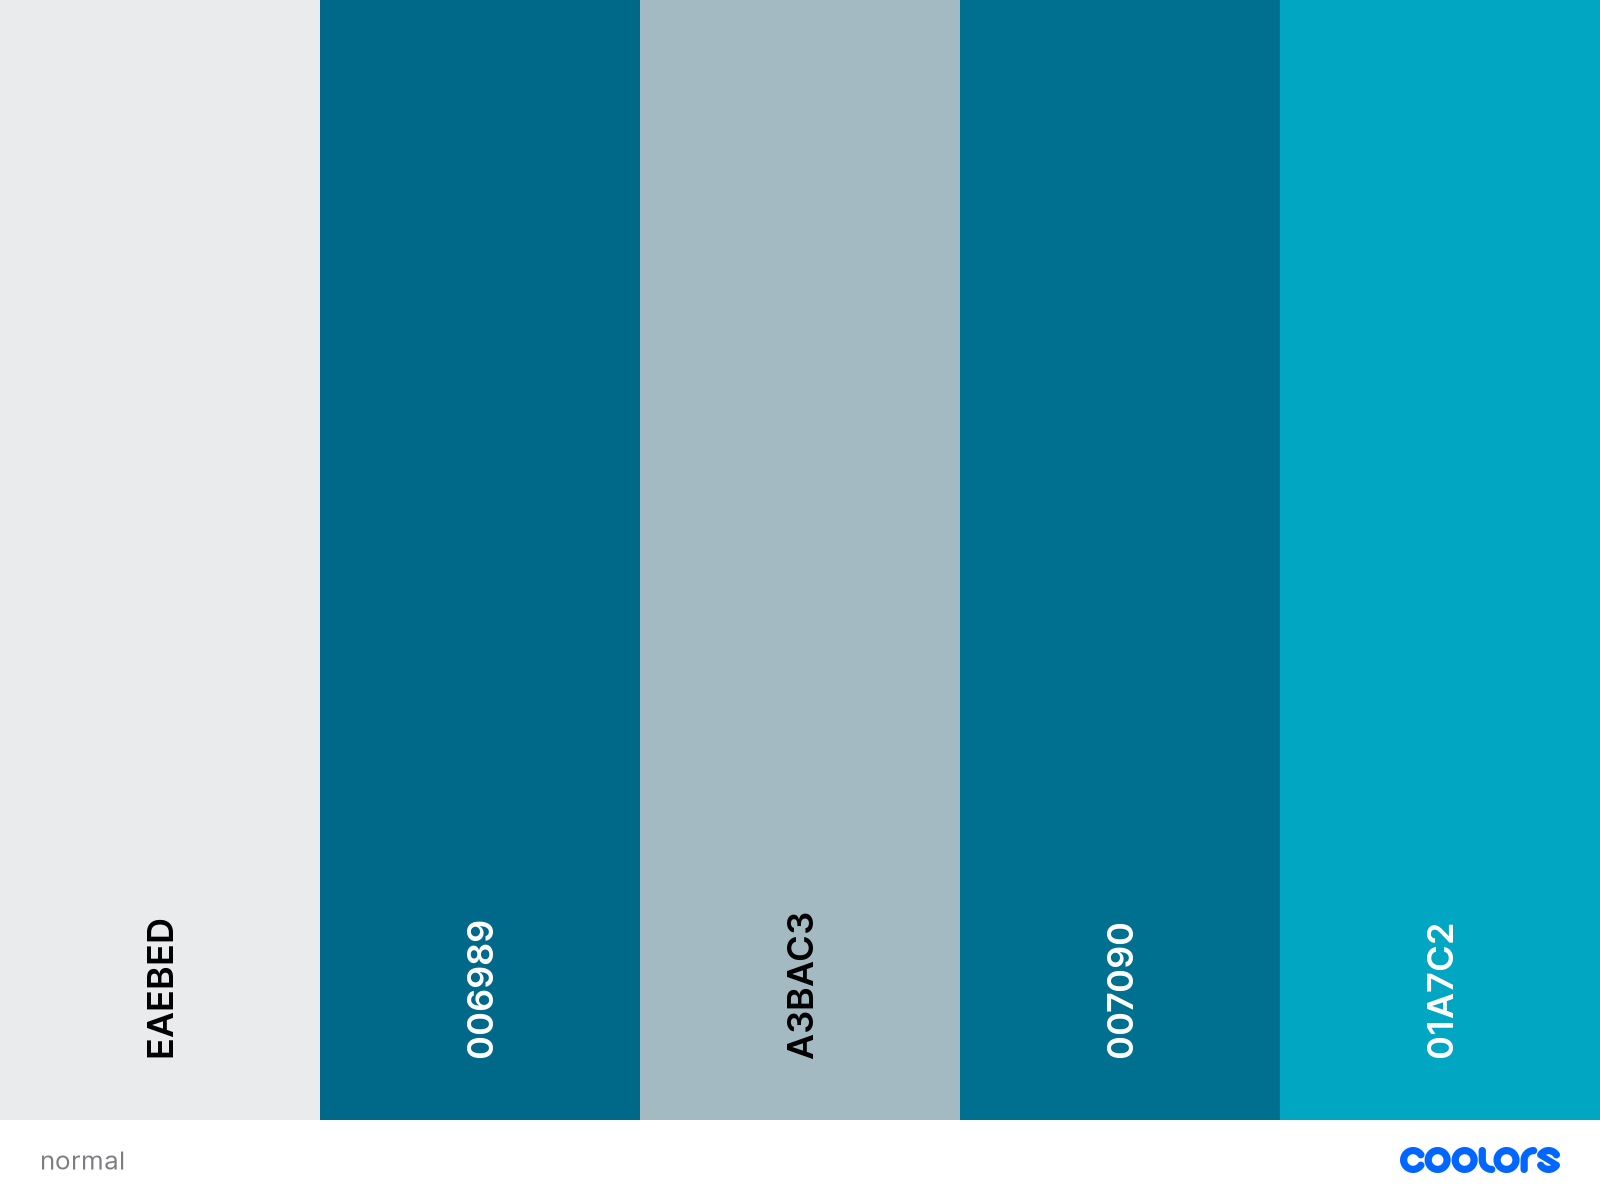
\includegraphics[scale=0.1]{normal} & 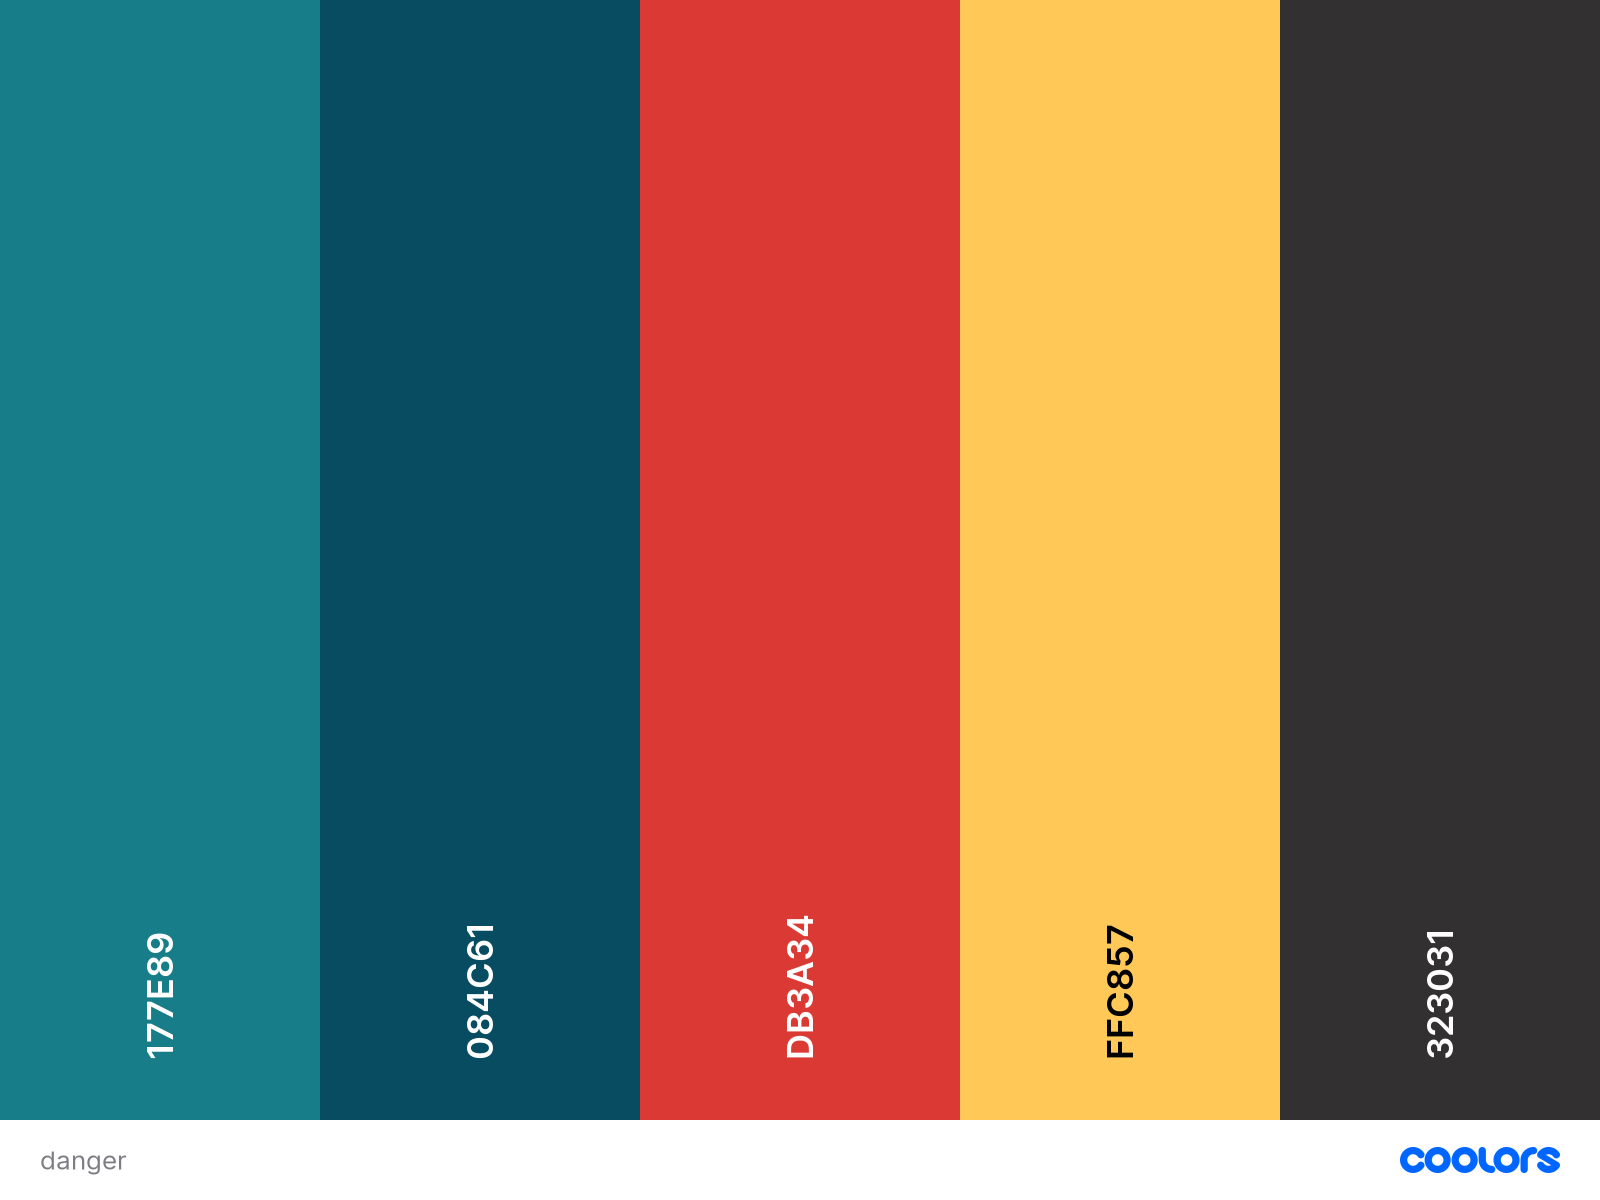
\includegraphics[scale=0.1]{danger}\\
Stealth (Danger, hidden)&Panic (Danger, low health)\\
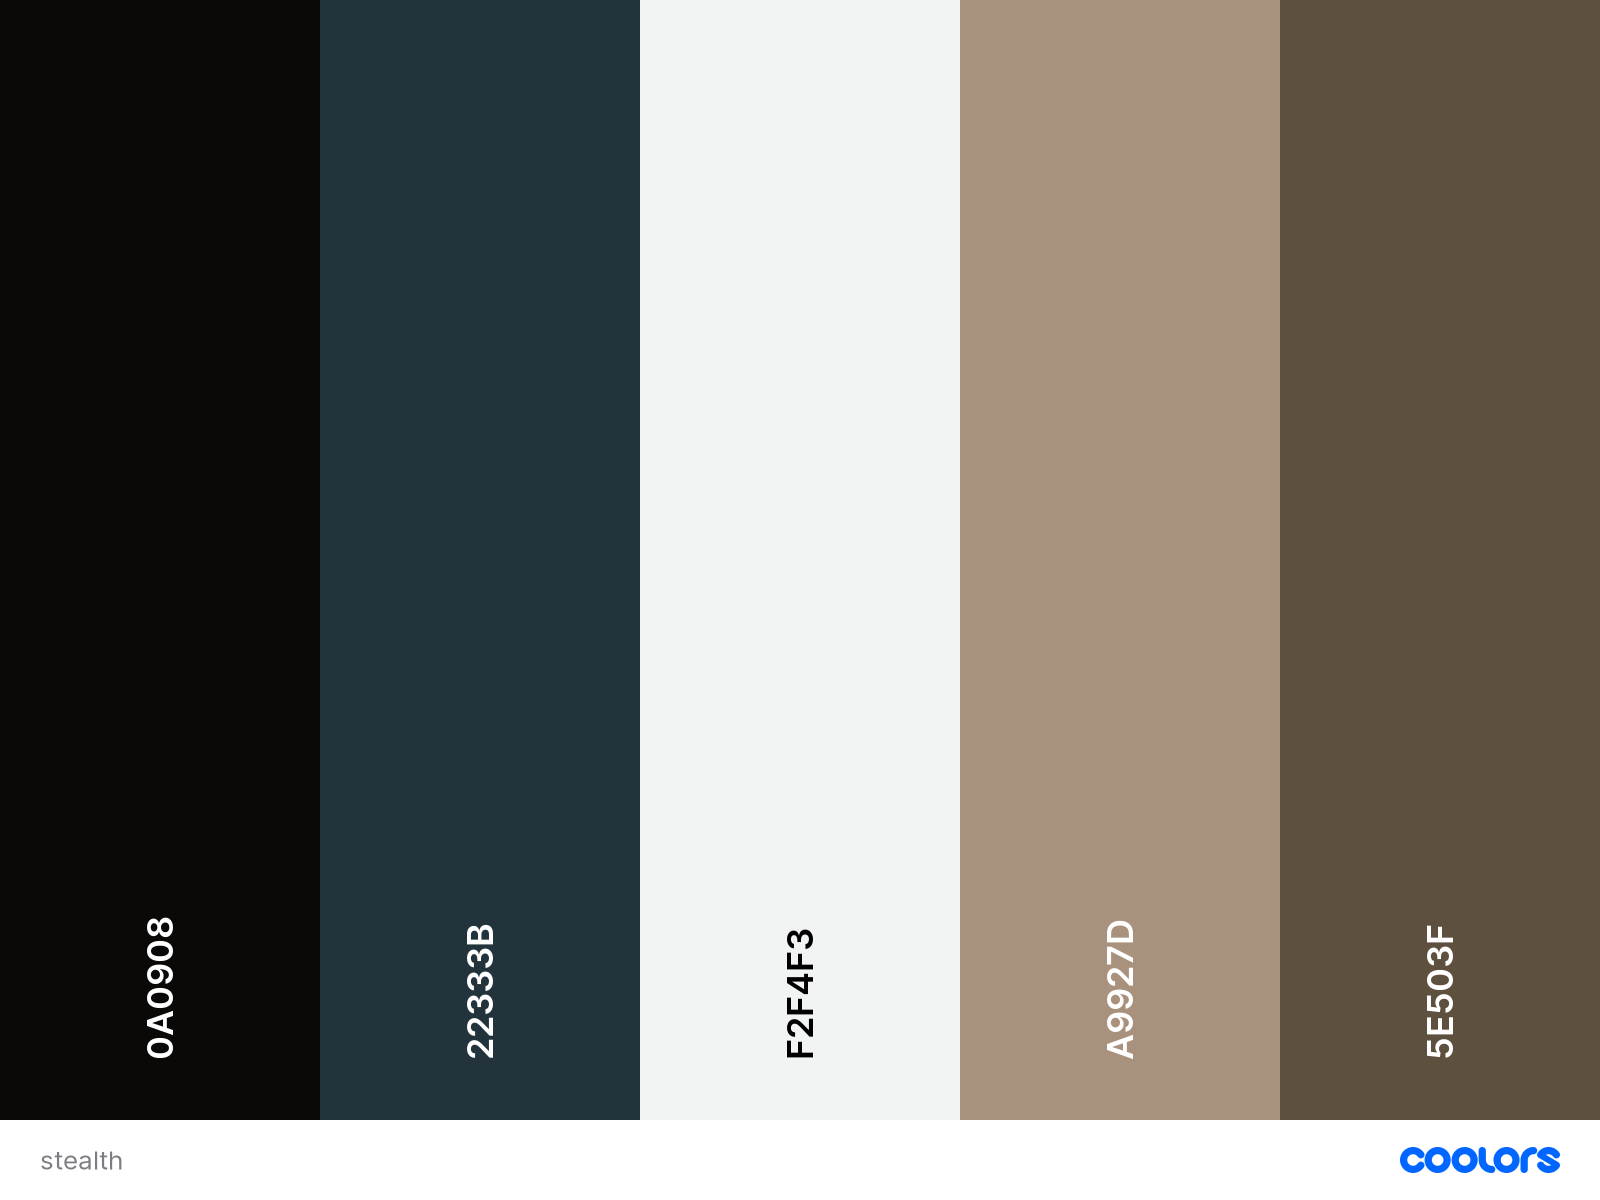
\includegraphics[scale=0.1]{stealth}&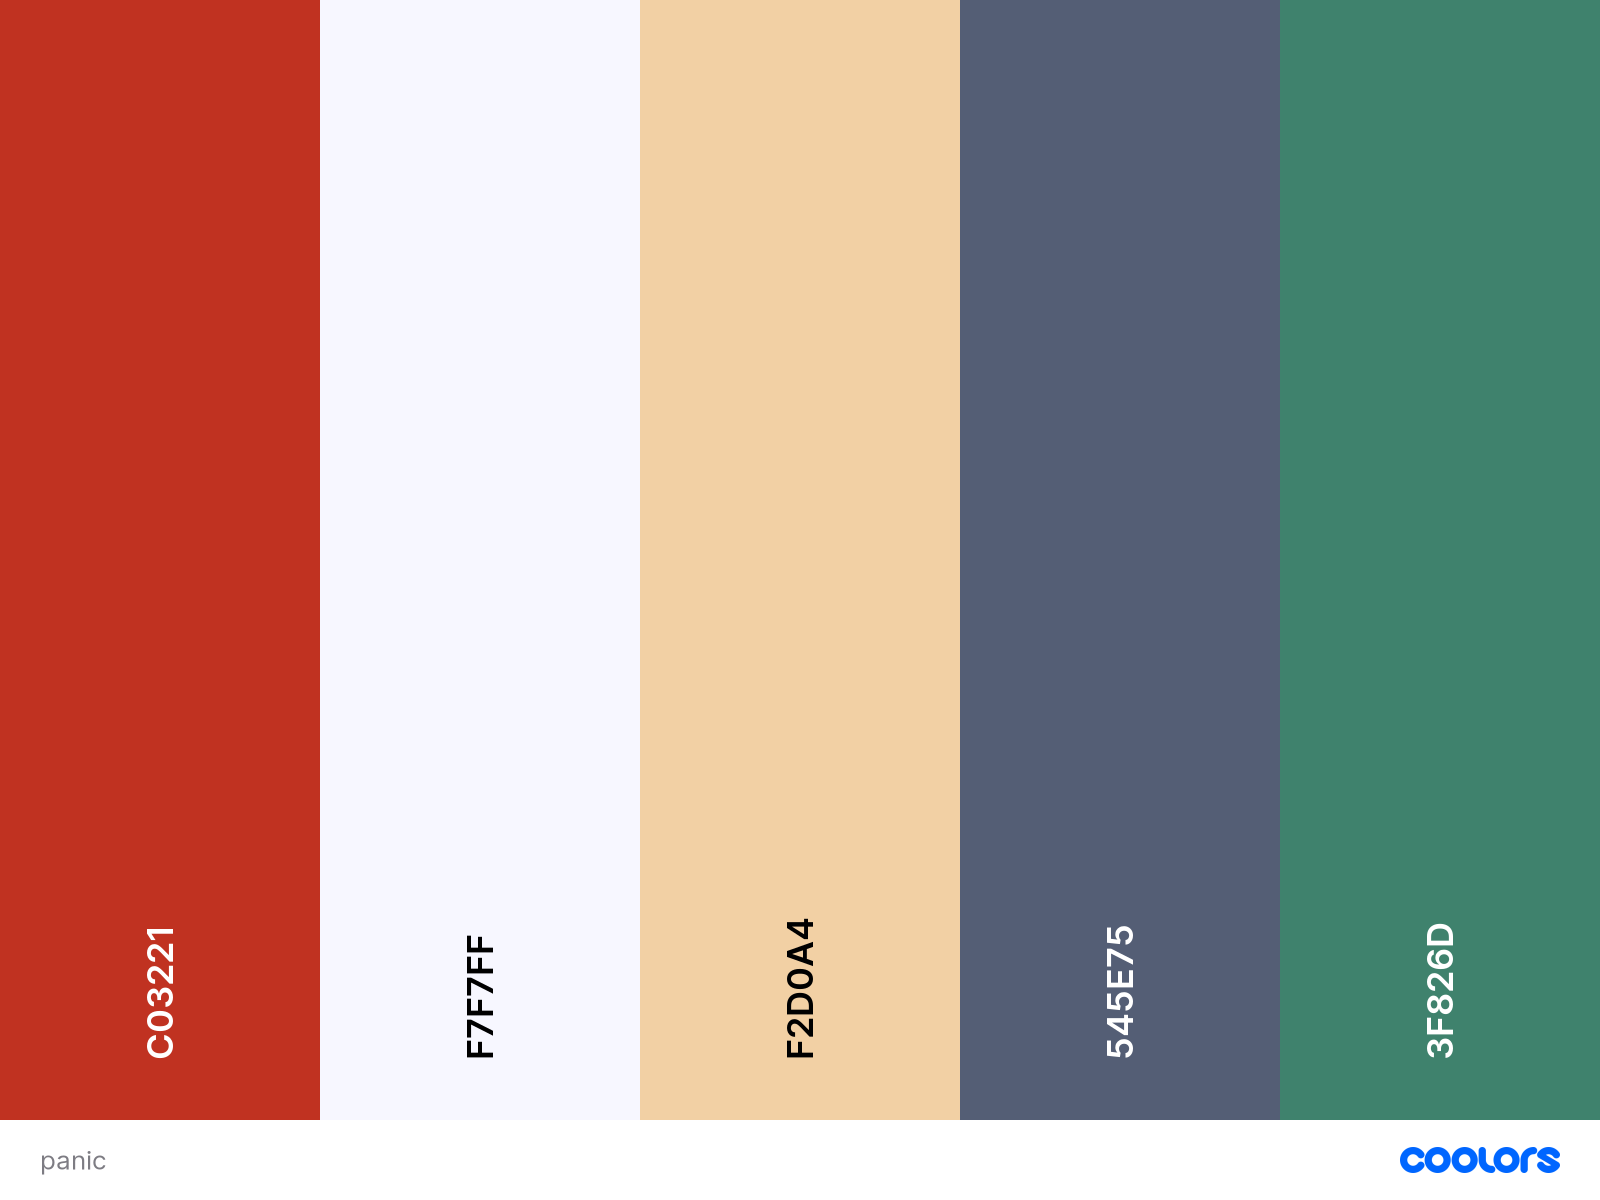
\includegraphics[scale=0.1]{panic}\\
Boss L(Boss, low health)&Boss W(Boss, boss hp low)\\
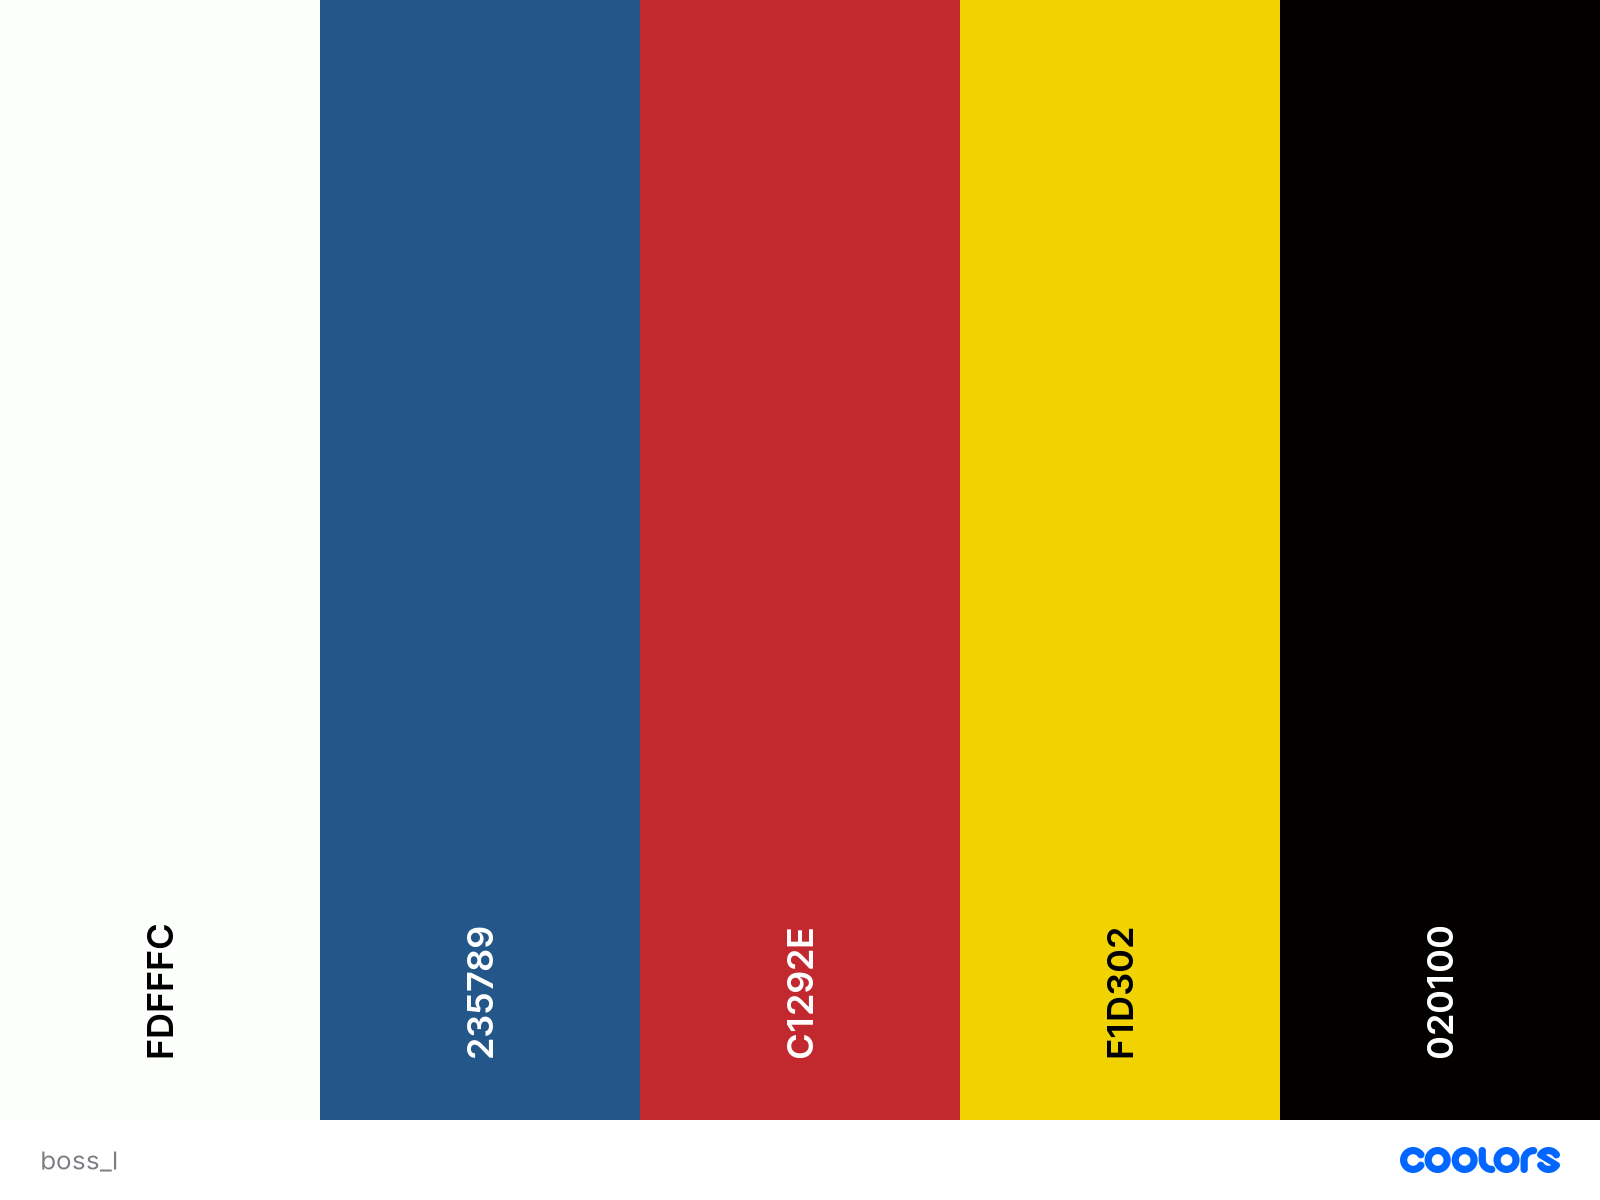
\includegraphics[scale=0.1]{boss_l}&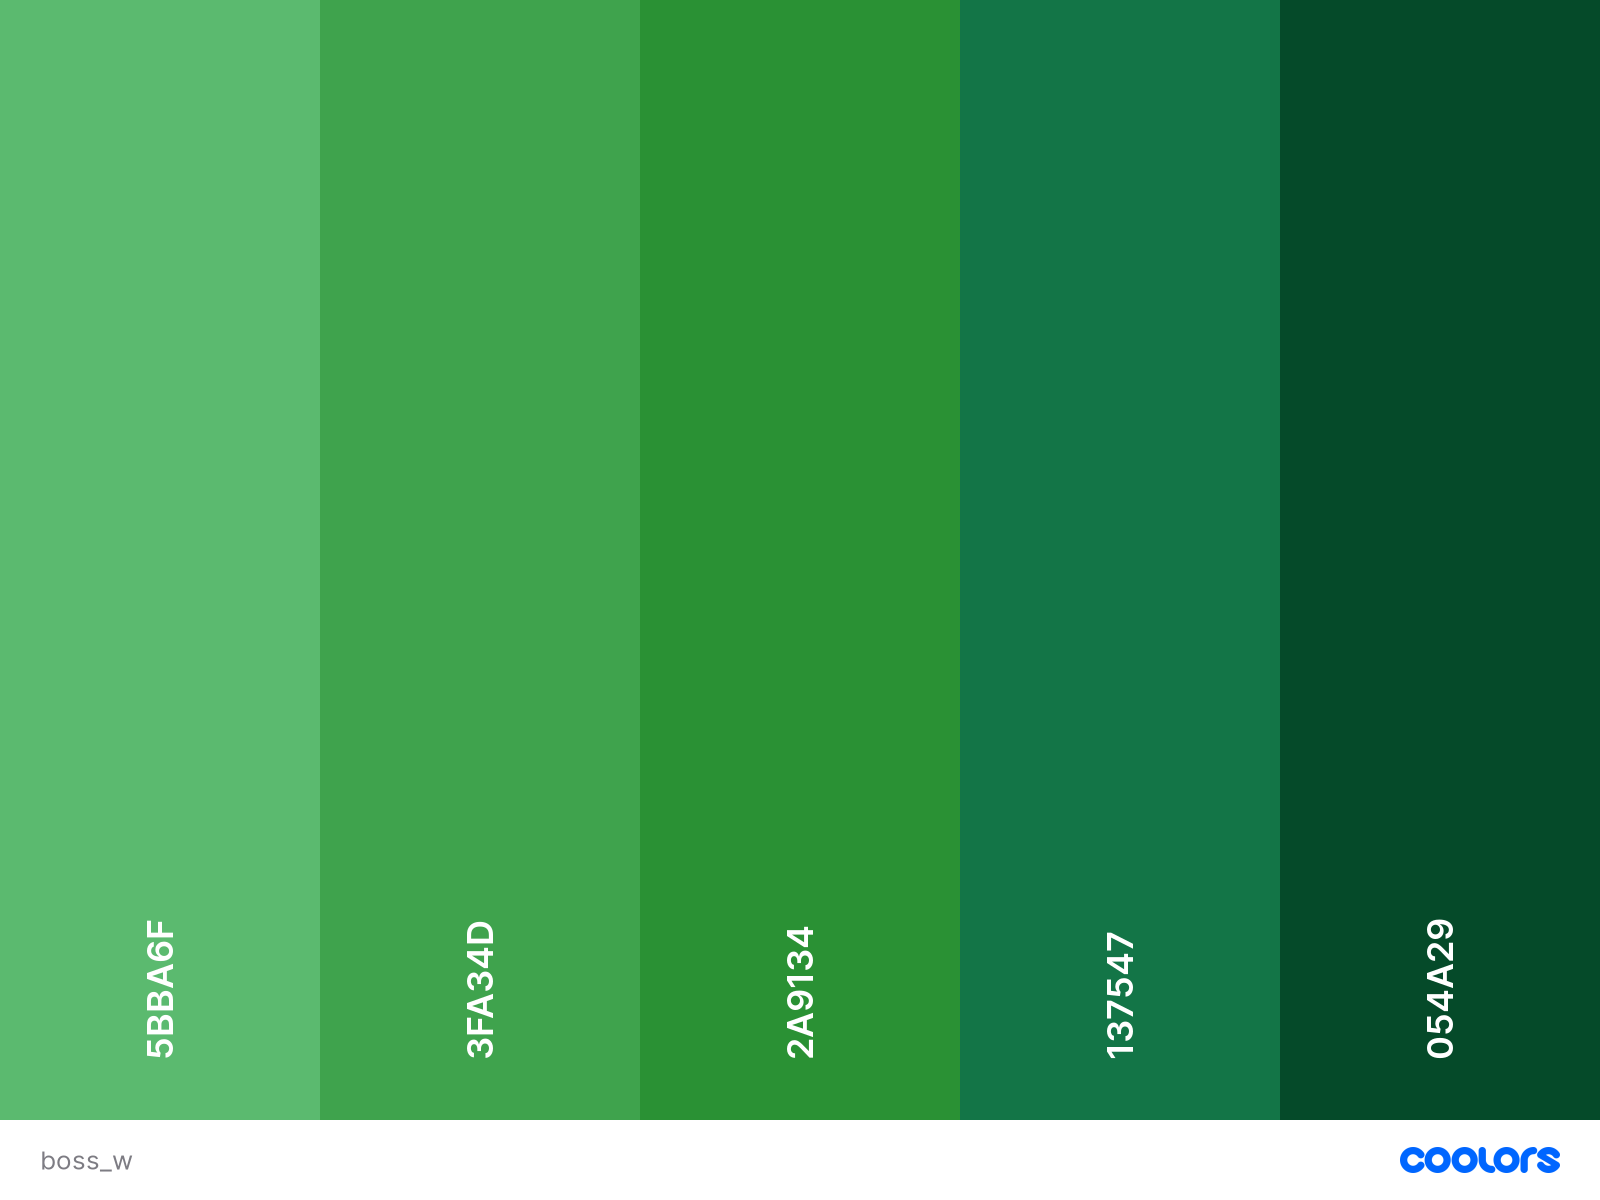
\includegraphics[scale=0.1]{boss_w}\\


\end{tabular}
\subsection{Lighting}
%Describe the lighting model/style your game will use. Include as many details as necessary, including anything custom you are doing to an existing lighing model, tricks you use to change how things are shaded or custom lighting systems / shaders you develop.
PBR-Shader dynamic realistic provided by FakeEngine3 (v. 1.12.2). 

\subsection{Mapping}
%Describe asthetic principles that should be kept when making maps. This may include setting, location, technical limitations, geometry stylisation and more. These principles should be detailed enough to describe your worlds shape and look so that someone making maps can keep the style consistent.
\subsubsection{Rough, jagged geometry}
Geometry should look purposefully rough and edged. Rounded corners should be avoided. Arches should be avoided.
\subsubsection{Limited draw distance, fog}
Game should have permanent fog covering up the limited draw distance of only 200 units. 
\subsection{User Interface}
%Outline a general overview of the User Interface. Describe how it will react to interactions, changes in game world etc. Provide an overview of the menu interfaces and anything else you want. its a good idea to include mockups, diagrams and other visualisations to explain it. Describe the general design idea behind how the UI should look. If you want to be very detailed, you can already specify color codes for UI elements, fonts to be used, icons to be used etc. This should be detailed enough so that UI remains consistent across the entire game. GENERAL TIP: If you need to use a value a lot (like a certain color or something), consider naming it at the first time using it and using the name (hereforth referred to as xxx) instead of pasting in the value itself everytime.
\subsubsection{Ingame-HUD}
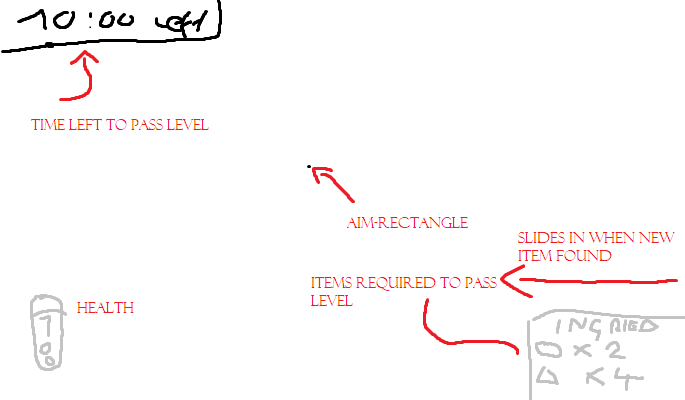
\includegraphics[scale=0.669]{mockup}\\
Lorem ipsum dolor sit amet, consectetur adipiscing elit, sed do eiusmod tempor incididunt ut labore et dolore magna aliqua. Ut enim ad minim veniam, quis nostrud exercitation ullamco laboris nisi ut aliquip ex ea commodo consequat. Duis aute irure dolor in reprehenderit in voluptate velit esse cillum dolore eu fugiat nulla pariatur. Excepteur sint occaecat cupidatat non proident, sunt in culpa qui officia deserunt mollit anim id est laborum.
\subsubsection{Main Menu}
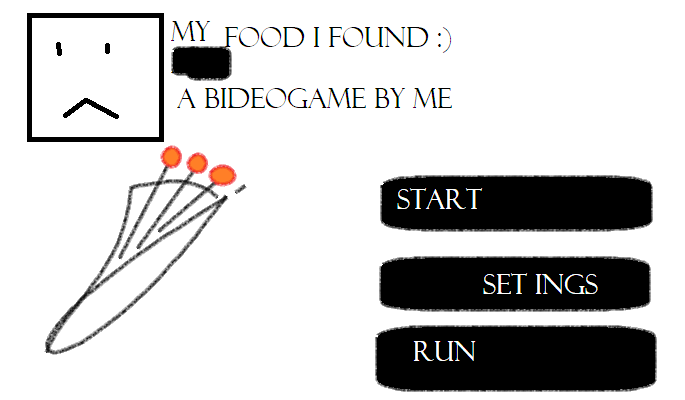
\includegraphics[scale=0.669]{mockup_mainmenu}\\
Lorem ipsum dolor sit amet, consectetur adipiscing elit, sed do eiusmod tempor incididunt ut labore et dolore magna aliqua. Ut enim ad minim veniam, quis nostrud exercitation ullamco laboris nisi ut aliquip ex ea commodo consequat. Duis aute irure dolor in reprehenderit in voluptate velit esse cillum dolore eu fugiat nulla pariatur. Excepteur sint occaecat cupidatat non proident, sunt in culpa qui officia deserunt mollit anim id est laborum.
%-----------------------------------------
\section{Technical Specifications}

\subsection{Supported Platforms}
\begin{itemize}
\item Windows
\item Linux
\end{itemize}

\subsection{Game Engine}
%The following section contains a utility analysis which aims to specify your requirements of the engine and its features in detail and end up helping you choose what engine to use. It is a pretty dry approach to picking your engine, but its a nice thing to try if you struggle picking the right engine for the job. If you have already decided to use a specific engine or can only really use one engine, please instead simply state and describe the engine in one or two paragraphs. If you are making your own game engine, you may find that specifying which features you need and how you plan on fullfilling them helps your development. The layout below is a suggestion for those who want to choose a premade engine. Please adapt or change it as needed. 

\subsubsection{Requirements}
\paragraph{Requirement 1}
this section is named requirement 1, however it really should be renamed to whatever requirement you have. Describe the requirement here in detail. If the requirement is self explanatory, you may omit the explanation. However, it is highly recommended to include a table detailing the rough criteria you will try and follow when assigning points in the analysis section of the document (see below)
\subparagraph{Points}
\begin{tabular}{c c}
Point Range & Description\\
5&Free\\
4&below 50 \euro\\
3-1&above 50 \euro
\end{tabular}

\paragraph{Requirement 2}
\subparagraph{Points}
\begin{tabular}{c c}
Point Range & Description\\
5&Lorem\\
4-1&Ipsum
\end{tabular}

\paragraph{Lorem ipsum}
Lorem ipsum dolor sit amet, consectetur adipiscing elit, sed do eiusmod tempor incididunt ut labore et dolore magna aliqua. Ut enim ad minim veniam, quis nostrud exercitation ullamco laboris nisi ut aliquip ex ea commodo consequat. Duis aute irure dolor in reprehenderit in voluptate velit esse cillum dolore eu fugiat nulla pariatur. Excepteur sint occaecat cupidatat non proident, sunt in culpa qui officia deserunt mollit anim id est laborum.
\subparagraph{Points}
\begin{tabular}{c c}
Point Range & Description\\
5&Lorem\\
4-3&Ipsum\\
2-1&dolor
\end{tabular}

\subsubsection{Variants}

\paragraph{Fake Engine 01}
%Use this section to introduce this engine in one or two paragraphs
Fake engine 01, developed by fake company in 1254 BC, is a game engine capable of 2D and 3D graphics using a PBR-Based rendering pipeline. Its mainly used by indie developers and is FOSS.

\paragraph{Fake Engine the second}
Lorem ipsum dolor sit amet, consectetur adipiscing elit, sed do eiusmod tempor incididunt ut labore et dolore magna aliqua. Ut enim ad minim veniam, quis nostrud exercitation ullamco laboris nisi ut aliquip ex ea commodo consequat. Duis aute irure dolor in reprehenderit in voluptate velit esse cillum dolore eu fugiat nulla pariatur. Excepteur sint occaecat cupidatat non proident, sunt in culpa qui officia deserunt mollit anim id est laborum.

\paragraph{Third one}
Lorem ipsum dolor sit amet, consectetur adipiscing elit, sed do eiusmod tempor incididunt ut labore et dolore magna aliqua. Ut enim ad minim veniam, quis nostrud exercitation ullamco laboris nisi ut aliquip ex ea commodo consequat. Duis aute irure dolor in reprehenderit in voluptate velit esse cillum dolore eu fugiat nulla pariatur. Excepteur sint occaecat cupidatat non proident, sunt in culpa qui officia deserunt mollit anim id est laborum.

\subsubsection{Analysis}
%This is the analysis section of the document. Here you will find out which engine should be the best choice for the project. Note that this analysis largely builds on subjective judgement and heavily relies on points being fairly awarded to the variants. Therefore, it  may not be correct all the time, but should be an aid in helping you choose an engine. Furthermore, it is recommended that you add another section where you detail why points were awarded to each variant in a certain way. This helps with understanding your scores later. However, you may omit this if you think that it won't be necessary. P = Points; W = Weighted Points (P*Weights); Variant with highest sum of W wins.
\begin{table}[ht]
\centering
\begin{tabular}{|c|c|c|c|c|c|c|c|}
\hline
Criteria & Weights & \multicolumn{2}{m{2cm}|}{Fake Engine 01} 
&  \multicolumn{2}{m{2cm}|}{Fake Engine the second}
& \multicolumn{2}{m{2cm}|}{Third one}\\
\hline
              &      & P & W   & P & W    & P & W\\
Requirement 1 & 50\% & 5 & 2.5 & 3 & 1.5  & 2 & 1 \\
Requirement 2 & 25\% & 2 & 0.5 & 1 & 0.25 & 4 & 1 \\
Lorem ipsum   & 25\% & 4 & 1   & 4 & 1    & 4 & 1\\
\hline
Sum           &      &11 & 4   & 8 & 2.75 & 10& 3\\
\hline
\end{tabular}
\caption{Utility analysis table}
\label{table:u_a}
\end{table}

\paragraph{Result}
According to Table \ref{table:u_a} Fake Engine 01 has the highest weighted score with 4 weighted points. Therefore it will be used for this project


\subsection{Rendering}
%Describe how your game will be rendered. Is it 2D/3D? What special rendering features does it use? are you going to make any custom rendering features? Feel free to add more subsubsections here to detail the rendering aspect of your game as much as needed. Asthetics and artstyle is covered in a different section
The game will use a standard PBR-based shading system provided by the game engine chosen. Graphically, the game consists mostly of 3D objects, however \emph{some characters are rendered in 2D. }
\subsubsection{2D in 3D}
To render 2D characters in a 3D environment, they will be \emph{drawn onto a 3D plane}. This plane will have a "\emph{billboard}" effect applied to it, which causes it to \emph{always face the camera}. Furthermore, the angle between the original forward vector of the plane and the look-vector of the plane (vector between the position of the camera and the position of the plane) will be calculated and the \emph{sprite modified to display a properly rotated version of the character.}

\subsection{Control Scheme}
%Describe the default control scheme for each platform
\subsubsection{Windows}
\begin{tabular}{|c|c|}
\hline
Key&Action\\
\hline
W&PLR\_FWD\\
S&PLR\_BCK\\
A&PLR\_L\\
D&PLR\_R\\
SPACEBAR&PLR\_JUMP\\
MOUSE1&PLR\_PRIM\\
MOUSE2&PLR\_SEC\\
\hline
\end{tabular}
%------------------------------------------

\section{Changelog}
%in this section, simply list any changes you have made to the document in enough detail so someone else, who knows nothing about the project, can tell what you did with a decent amount of accuracy. The first entry may simply be "Initial document"/"Initial version" or whatever else you like. REMEMBER TO INCLUDE A DATE FOR EACH ENTRY. This date may help link the versions to commits in a version control system, or simply make understanding the timeline of development for your game a bit easier (for example you may want to find out roughly when you first introduced an idea into your game officially)
\subsection{Version 0.0.1 - unfinished change}
\begin{itemize}
\item Changed title from 'gunpowder dream' to 'shoppatomic'
\item Removed primary mention of old store name. Come up with a new one (TODO)
\end{itemize}
Notice: The initial version of this document was filled with some content on the first pages, however I failed to denote this in the changelog. This is the first change made after the initial filling of the document with some basic content a while ago. Refer to git repository for more details.

\date{June 04, 2021}
\end{document}